% ============================================================
%  SmartInterview — Full Project Documentation
%  Compile with: pdflatex SmartInterview_Documentation.tex
%  (run twice for correct cross-references and TOC)
% ============================================================
\documentclass[12pt,a4paper]{article}

% ── Packages ────────────────────────────────────────────────
\usepackage[margin=2.5cm]{geometry}
\usepackage{hyperref}
\usepackage{graphicx}
\usepackage{booktabs}
\usepackage{tabularx}
\usepackage{longtable}
\usepackage{array}
\usepackage{xcolor}
\usepackage{listings}
\usepackage{fancyhdr}
\usepackage{titlesec}
\usepackage{enumitem}
\usepackage{amsmath}
\usepackage{microtype}
\usepackage{parskip}
\usepackage{caption}
\usepackage{subcaption}
\usepackage{float}
\usepackage{tcolorbox}
\usepackage{mdframed}
\usepackage{tikz}
\usetikzlibrary{shapes.geometric, arrows.meta, positioning, fit, backgrounds}
\usepackage{fontenc}
\usepackage{inputenc}

% ── Colors ──────────────────────────────────────────────────
\definecolor{accent}{RGB}{79,142,247}
\definecolor{accentdark}{RGB}{50,100,200}
\definecolor{codebg}{RGB}{245,247,250}
\definecolor{codefg}{RGB}{30,40,60}
\definecolor{green}{RGB}{22,163,74}
\definecolor{red}{RGB}{220,38,38}
\definecolor{yellow}{RGB}{180,140,20}
\definecolor{purple}{RGB}{124,58,237}
\definecolor{lightgray}{RGB}{230,232,238}
\definecolor{warningbg}{RGB}{255,251,235}
\definecolor{warningborder}{RGB}{251,191,36}
\definecolor{infobg}{RGB}{239,246,255}
\definecolor{infoborder}{RGB}{147,197,253}

% ── Code listings style ─────────────────────────────────────
\lstset{
  backgroundcolor=\color{codebg},
  basicstyle=\ttfamily\small,
  keywordstyle=\color{accentdark}\bfseries,
  commentstyle=\color{green}\itshape,
  stringstyle=\color{red},
  numberstyle=\tiny\color{gray},
  numbers=left,
  stepnumber=1,
  numbersep=8pt,
  frame=single,
  framerule=0.4pt,
  rulecolor=\color{lightgray},
  breaklines=true,
  breakatwhitespace=true,
  showstringspaces=false,
  tabsize=2,
  captionpos=b,
  aboveskip=8pt,
  belowskip=8pt,
}
\lstdefinestyle{bash}{language=bash,morekeywords={pip,uvicorn,npm,python}}
\lstdefinestyle{python}{language=Python}

% ── Info/Warning boxes ──────────────────────────────────────
\tcbuselibrary{skins,breakable}
\newtcolorbox{infobox}[1][]{
  colback=infobg, colframe=infoborder, fonttitle=\bfseries,
  title=#1, breakable, left=6pt, right=6pt, top=4pt, bottom=4pt
}
\newtcolorbox{warningbox}[1][]{
  colback=warningbg, colframe=warningborder, fonttitle=\bfseries,
  title=#1, breakable, left=6pt, right=6pt, top=4pt, bottom=4pt
}

% ── Header / footer ─────────────────────────────────────────
\pagestyle{fancy}
\fancyhf{}
\fancyhead[L]{\small\textcolor{gray}{SmartInterview --- Technical Documentation}}
\fancyhead[R]{\small\textcolor{gray}{May 2026}}
\fancyfoot[C]{\small\thepage}
\renewcommand{\headrulewidth}{0.4pt}

% ── Title formatting ────────────────────────────────────────
\titleformat{\section}{\large\bfseries\color{accentdark}}{}{0pt}{\thesection\quad}[\vspace{2pt}\hrule\vspace{4pt}]
\titleformat{\subsection}{\normalsize\bfseries\color{accent}}{}{0pt}{\thesubsection\quad}
\titleformat{\subsubsection}{\normalsize\bfseries}{}{0pt}{\thesubsubsection\quad}

% ── TikZ styles ─────────────────────────────────────────────
\tikzset{
  box/.style={rectangle, rounded corners=4pt, draw=accent, fill=infobg, minimum width=2.6cm, minimum height=0.7cm, font=\small, align=center},
  bigbox/.style={rectangle, rounded corners=4pt, draw=accentdark, fill=infobg, minimum width=3.2cm, minimum height=0.85cm, font=\small\bfseries, align=center},
  greenbox/.style={rectangle, rounded corners=4pt, draw=green, fill=green!8, minimum width=2.6cm, minimum height=0.7cm, font=\small, align=center},
  arrow/.style={-Stealth, thick, color=accentdark},
}

% ── Document ─────────────────────────────────────────────────
\begin{document}

% ── Title page ───────────────────────────────────────────────
\begin{titlepage}
  \centering
  \vspace*{3cm}
  {\Huge\bfseries\color{accentdark} SmartInterview}\\[0.5em]
  {\large\color{accent} AI-Powered Personalized Interview Preparation Platform}\\[3cm]

  \begin{tabular}{rl}
    \textbf{Author}   & Ahmad Yarkhan \\[4pt]
    \textbf{Version}  & 1.0 \\[4pt]
    \textbf{Date}     & May 2026 \\[4pt]
    \textbf{Status}   & Testing Phase \\[4pt]
  \end{tabular}

  \vfill
  \hrule\vspace{8pt}
  {\small\color{gray}
    Full-stack AI system --- FastAPI backend $\cdot$ React frontend $\cdot$
    Gemini LLM $\cdot$ Faster-Whisper $\cdot$ Ensemble ML
  }
\end{titlepage}

\tableofcontents
\newpage

% ╔══════════════════════════════════════════════════════════╗
% ║  1. ABSTRACT                                             ║
% ╚══════════════════════════════════════════════════════════╝
\section{Abstract}

SmartInterview is a full-stack, AI-powered interview preparation platform that provides a realistic, personalized mock-interview experience entirely in the browser. The system accepts a candidate's r\'esum\'e, infers their technical profile using natural language processing, and assembles a tailored set of 12 interview questions drawn from two complementary sources: a curated question bank retrieved via semantic search, and questions generated directly by a large language model (LLM). The interview is delivered in an audio-first format: questions are read aloud by a text-to-speech engine, the candidate responds by voice, and their speech is transcribed by an ASR model before being scored by the LLM. In parallel, a separately trained ensemble classifier analyzes acoustic features of each spoken response to estimate the candidate's level of vocal confidence.

The system addresses three core research challenges: (1)~how to generate interview questions that are simultaneously relevant to a domain, personalized to the candidate's actual experience, and appropriately difficulty-distributed; (2)~how to score open-ended spoken answers reliably without human annotators; and (3)~how to classify vocal confidence from a very small, self-collected dataset that suffered from class imbalance. The third challenge led to the original contribution of this project: the self-recording and automated feature extraction of 42 unconfident voice samples to augment an existing dataset, followed by the training of a four-model soft-voting ensemble that achieved 88\% accuracy and a ROC-AUC of 0.927 on held-out test data.

% ╔══════════════════════════════════════════════════════════╗
% ║  2. PROJECT SUMMARY                                      ║
% ╚══════════════════════════════════════════════════════════╝
\section{Project Summary}

\subsection{Motivation}
Traditional interview preparation relies on mock interviews with human partners, flashcard memorization, or reading generic question lists. None of these approaches adapt to a specific candidate's background, provide instant feedback, or analyze non-verbal cues such as vocal confidence. SmartInterview was built to close this gap by combining retrieval-augmented generation, LLM-based evaluation, and classical machine learning in a single, deployable web application.

\subsection{Core Capabilities}
\begin{itemize}[leftmargin=1.5em]
  \item \textbf{Resume-aware question generation} --- questions reference the candidate's actual projects, technologies, and companies.
  \item \textbf{Multi-source question assembly} --- dataset questions are retrieved semantically and personalized; additional project-specific questions are generated by Gemini; HR behavioral questions are sampled separately.
  \item \textbf{Voice-first interview interface} --- questions are read aloud; candidates record spoken answers; browser MediaRecorder captures audio.
  \item \textbf{Whisper-based transcription} --- faster-whisper \texttt{medium.en} transcribes recorded audio with high accuracy, and the transcript is used for LLM scoring (replacing unreliable browser speech recognition).
  \item \textbf{LLM answer scoring} --- Gemini evaluates answers on three angles (conceptual, technical, completeness) and produces natural-language feedback.
  \item \textbf{Vocal confidence analysis} --- a four-model ensemble classifier predicts whether each spoken response sounds ``Confident'' or ``Unconfident'' and returns a 1--10 score.
  \item \textbf{Comprehensive final report} --- per-question breakdowns, category aggregates, and confidence scores are compiled into an interactive report.
\end{itemize}

\subsection{Development Timeline}
The project was implemented in four phases: initial full-stack setup with RAG-based question generation and cosine-similarity scoring (commit \texttt{03a91a3}); integration of the voice confidence ML model and feature extraction pipeline (\texttt{f308a86}); addition of Whisper transcription and audio-based Gemini scoring (\texttt{b6c027d}); and UX refinements including per-question score removal, improved loading screens, and TTS provider switching (\texttt{c640551}, \texttt{ef8bab3}).

% ╔══════════════════════════════════════════════════════════╗
% ║  3. SYSTEM ARCHITECTURE                                  ║
% ╚══════════════════════════════════════════════════════════╝
\section{System Architecture}

\subsection{High-Level Architecture}

\begin{figure}[H]
\centering
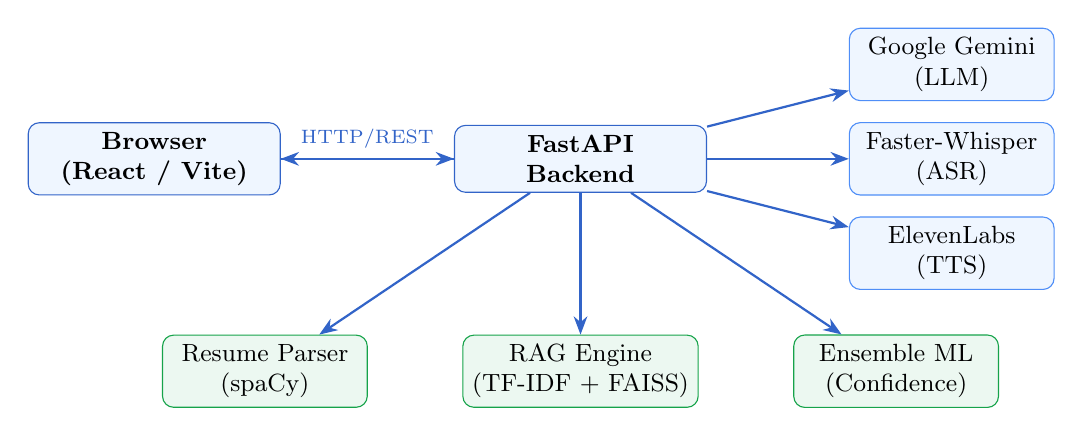
\begin{tikzpicture}[node distance=0.8cm and 1.2cm]
  % Frontend
  \node[bigbox] (browser) {Browser\\(React / Vite)};
  % Backend
  \node[bigbox, right=2.2cm of browser] (api) {FastAPI\\Backend};
  % External services
  \node[box, above right=0.3cm and 1.8cm of api] (gemini) {Google Gemini\\(LLM)};
  \node[box, right=1.8cm of api] (whisper) {Faster-Whisper\\(ASR)};
  \node[box, below right=0.3cm and 1.8cm of api] (elevenlabs) {ElevenLabs\\(TTS)};
  % Internal modules
  \node[greenbox, below=1.8cm of api] (rag) {RAG Engine\\(TF-IDF + FAISS)};
  \node[greenbox, left=1.2cm of rag] (parser) {Resume Parser\\(spaCy)};
  \node[greenbox, right=1.2cm of rag] (ml) {Ensemble ML\\(Confidence)};

  % Arrows browser <-> api
  \draw[arrow] (browser) -- node[above,font=\scriptsize]{HTTP/REST} (api);
  \draw[arrow] (api) -- (browser);
  % api -> external
  \draw[arrow] (api) -- (gemini);
  \draw[arrow] (api) -- (whisper);
  \draw[arrow] (api) -- (elevenlabs);
  % api -> internal
  \draw[arrow] (api) -- (rag);
  \draw[arrow] (api) -- (parser);
  \draw[arrow] (api) -- (ml);
\end{tikzpicture}
\caption{High-level system architecture. The FastAPI backend orchestrates all AI and ML services.}
\end{figure}

\subsection{Directory Structure}

\begin{lstlisting}[language=bash, numbers=none]
SmartInterview/
|-- backend/
|   |-- main.py                # FastAPI server, routes, session store
|   |-- gemini_client.py       # Gemini API wrapper (Q gen + scoring)
|   |-- feature_extractor.py   # Audio feature extraction + ML prediction
|   |-- embedding_engine.py    # TF-IDF vectorizer + FAISS index
|   |-- resume_parser.py       # spaCy NER + regex resume parser
|   |-- scorer.py              # Local cosine/keyword scorer (backup)
|   |-- data_loader.py         # Question bank loader + indexer
|   |-- text_extractor.py      # PDF/DOCX/TXT text extraction
|   |-- requirements.txt
|   |-- models/
|   |   |-- ensemble_confidence_model.joblib
|   |   `-- features_list.joblib
|   |-- data/
|   |   `-- master_questions.csv
|   `-- training/
|       |-- ConfidenceAnalysis.ipynb      # Model training
|       `-- UnconfidentVms_Preprocess.ipynb  # Dataset augmentation
`-- frontend/
    |-- package.json
    |-- vite.config.js
    `-- src/
        |-- App.jsx
        |-- index.css
        |-- hooks/useInterview.js
        |-- utils/api.js
        `-- components/
            |-- UploadScreen.jsx
            |-- ReadyScreen.jsx
            |-- InterviewScreen.jsx
            |-- ReportScreen.jsx
            |-- ProfileStrip.jsx
            |-- ConfidenceTestPage.jsx
            `-- QuestionsPage.jsx
\end{lstlisting}

\subsection{Data Flow Overview}

The end-to-end flow for a single interview session is:

\begin{enumerate}[leftmargin=2em]
  \item User uploads r\'esum\'e PDF/DOCX $\rightarrow$ text extracted, session created.
  \item User optionally enters job role and job description.
  \item Backend assembles 12 questions via the 3-source pipeline (Section~\ref{sec:qgen}).
  \item For each question: TTS reads it aloud; user records spoken answer.
  \item Audio blob sent to \texttt{/api/confidence}: Whisper transcribes, 6 features extracted, ensemble model predicts confidence; transcript returned.
  \item Whisper transcript sent to \texttt{/api/score}: Gemini evaluates against model answer; 3-angle scores returned.
  \item After all questions, \texttt{/api/report} aggregates all answers into a final report.
\end{enumerate}

% ╔══════════════════════════════════════════════════════════╗
% ║  4. TECHNOLOGY STACK                                     ║
% ╚══════════════════════════════════════════════════════════╝
\section{Technology Stack}

\begin{table}[H]
\centering
\caption{Complete technology stack}
\small
\begin{tabularx}{\textwidth}{l l X}
\toprule
\textbf{Layer} & \textbf{Technology} & \textbf{Role / Notes} \\
\midrule
\multicolumn{3}{l}{\textit{Backend}} \\
& FastAPI 0.111 & Async REST API framework; handles all routes \\
& Uvicorn & ASGI server for FastAPI \\
& Python 3.12 & Runtime \\
& pydantic & Request/response validation \\
& python-dotenv & \texttt{.env} configuration loading (\texttt{override=True}) \\
& aiofiles & Async file I/O \\
& httpx & Async HTTP client for ElevenLabs TTS proxy \\
\midrule
\multicolumn{3}{l}{\textit{NLP \& Text}} \\
& spaCy (en\_core\_web\_sm) & Named entity recognition for resume name extraction \\
& pdfplumber & PDF text extraction (layout-aware) \\
& python-docx & DOCX paragraph extraction \\
& google-generativeai & Gemini API client (question generation + scoring) \\
\midrule
\multicolumn{3}{l}{\textit{Retrieval}} \\
& scikit-learn TF-IDF & Text vectorization (8000 features, 1--2 ngrams) \\
& FAISS (IndexFlatIP) & Fast approximate nearest-neighbor search \\
& numpy & Vector math, L2 normalization \\
\midrule
\multicolumn{3}{l}{\textit{Audio \& Speech}} \\
& faster-whisper & Whisper \texttt{medium.en} via CTranslate2; CUDA/CPU fallback \\
& pydub & Audio format conversion (webm/m4a $\rightarrow$ wav) \\
& ffmpeg & Audio codec backend (required by pydub) \\
\midrule
\multicolumn{3}{l}{\textit{Machine Learning}} \\
& scikit-learn 1.6.1 & LogisticRegression, RandomForest, AdaBoost, VotingClassifier \\
& XGBoost & Gradient boosting classifier \\
& joblib & Model serialization/deserialization \\
& pandas & Feature dataframe construction \\
\midrule
\multicolumn{3}{l}{\textit{Frontend}} \\
& React 18.3.1 & UI framework (hooks-based, no class components) \\
& Vite 5.3.1 & Build tool; dev server with \texttt{/api} proxy \\
& axios 1.7.2 & HTTP client with 60 s / 120 s timeouts \\
& react-dropzone 14.2.3 & Drag-and-drop file upload \\
& Web Speech API & Silent browser speech recognition (text fallback only) \\
& MediaRecorder API & In-browser audio capture (webm blob) \\
& Web Speech Synthesis & Browser TTS (fallback when ElevenLabs not configured) \\
\midrule
\multicolumn{3}{l}{\textit{External APIs}} \\
& Google Gemini 2.0 Flash & LLM for question generation + answer scoring \\
& ElevenLabs (eleven\_turbo\_v2) & Realistic text-to-speech (optional) \\
\bottomrule
\end{tabularx}
\end{table}

% ╔══════════════════════════════════════════════════════════╗
% ║  5. IMPLEMENTATION DETAILS                               ║
% ╚══════════════════════════════════════════════════════════╝
\section{Implementation Details}

\subsection{API Endpoints (\texttt{main.py})}

\begin{table}[H]
\centering
\caption{Backend REST API endpoints}
\small
\begin{tabularx}{\textwidth}{l l X}
\toprule
\textbf{Method} & \textbf{Path} & \textbf{Purpose} \\
\midrule
POST & \texttt{/api/upload-resume} & Accept PDF/DOCX/TXT, extract text, create session \\
GET  & \texttt{/api/questions/\{session\_id\}} & Assemble and return 12 personalized questions \\
POST & \texttt{/api/score} & Score a single answer via Gemini \\
GET  & \texttt{/api/report/\{session\_id\}} & Compute and return final report \\
POST & \texttt{/api/confidence} & Transcribe audio + analyze confidence \\
POST & \texttt{/api/tts} & ElevenLabs TTS proxy; returns MP3 stream \\
GET  & \texttt{/api/health} & System status, session count, RAG readiness \\
GET  & \texttt{/api/debug/chunks/\{session\_id\}} & Expose resume chunks and retrieval sources \\
DELETE & \texttt{/api/session/\{session\_id\}} & Delete session from in-memory store \\
\bottomrule
\end{tabularx}
\end{table}

\subsection{Session Management}

SmartInterview uses a simple in-memory session store (a Python \texttt{dict}) keyed by UUID. Each session stores:

\begin{lstlisting}[style=python, numbers=none]
sessions[session_id] = {
    "resume_text": str,          # raw extracted text
    "filename": str,             # original upload filename
    "job_role": str,             # optional target role
    "job_description": str,      # optional pasted JD
    "questions": list[dict],     # assembled question objects
    "answers": list[dict],       # scored answer records
    "debug_chunks": dict,        # resume section chunks
    "debug_retrieval": dict,     # dataset/project/HR question sources
}
\end{lstlisting}

Sessions persist for the lifetime of the server process and are explicitly deleted on reset. There is no database or cache layer.

\subsection{Resume Parsing (\texttt{resume\_parser.py})}

The parser uses a combination of regex section detection and spaCy NER:

\begin{enumerate}[leftmargin=2em]
  \item \textbf{Text extraction} via \texttt{text\_extractor.py}: PDF $\rightarrow$ \texttt{pdfplumber} (layout-aware); DOCX $\rightarrow$ \texttt{python-docx} paragraphs; TXT $\rightarrow$ UTF-8 decode.
  \item \textbf{Name extraction}: spaCy \texttt{en\_core\_web\_sm} PERSON entity on the first 500 characters; fallback to first non-special-character line.
  \item \textbf{Title extraction}: keyword-pattern regex on lines near the name (engineer, developer, architect, scientist, analyst, manager, \ldots).
  \item \textbf{Skills extraction}: section header detection via regex + scan against a \texttt{KNOWN\_SKILLS} set.
  \item \textbf{Experience, education, projects}: regex section boundaries (case-insensitive headers); structured into dicts with role, company, duration, highlights.
  \item \textbf{Category weighting}: each of the 11 canonical categories has a keyword map; weight formula:
  \[
    w_c = \min\!\left(1.0,\ 0.10 + \frac{\text{matches}(c)}{\max\!\left(\lvert\text{keywords}(c)\rvert \cdot 0.3,\ 1\right)} \times 0.90\right)
  \]
  HR \& Behavioral receives a fixed weight of 0.50 for all candidates.
\end{enumerate}

\subsection{Question Generation Pipeline}
\label{sec:qgen}

\subsubsection{Category Inference}

When no job description is provided, Gemini is called with a short prompt to infer 3--5 relevant technical categories from the r\'esum\'e text, capped to the 11 canonical categories.

\subsubsection{Dataset Question Retrieval}

\begin{enumerate}[leftmargin=2em]
  \item Filter categories with weight $\geq 0.3$ (or take the top 3 if all weights are below threshold).
  \item For each selected category: embed the r\'esum\'e (first 3000 characters) and all questions in that category using the TF-IDF engine; rank by cosine similarity; take the top 2 questions.
  \item Collect up to 5 dataset questions total across categories.
\end{enumerate}

\subsubsection{Combined Gemini Call: Personalize + Generate}

A single Gemini call handles two tasks simultaneously (\texttt{\_COMBINED\_QUESTION\_PROMPT}):

\begin{description}[leftmargin=2em]
  \item[Task 1 --- Personalize] Rewrite each of the 5 retrieved dataset questions to reference a specific project, technology, or decision from the candidate's r\'esum\'e. The core concept, category, and difficulty are preserved.
  \item[Task 2 --- Generate] Create 4 new questions grounded in the \textit{Projects} section of the r\'esum\'e. Each question must target a concrete technical decision or implementation detail from a named project.
\end{description}

The response is a JSON object with two arrays: \texttt{"dataset"} and \texttt{"project"}.

\subsubsection{HR Questions}

3 behavioral questions are sampled randomly from the dataset (\texttt{category = "HR \& Behavioral"}). These have \texttt{has\_answer = false} and no model answer.

\subsubsection{Assembly and Deduplication}

The three batches (5 personalized + 4 project + 3 HR = 12) are concatenated. A TF-IDF cosine deduplication step removes any question whose cosine similarity to an earlier question exceeds 0.70. Questions are re-indexed (\texttt{q1}--\texttt{q12}) and cached in the session.

\begin{figure}[H]
\centering
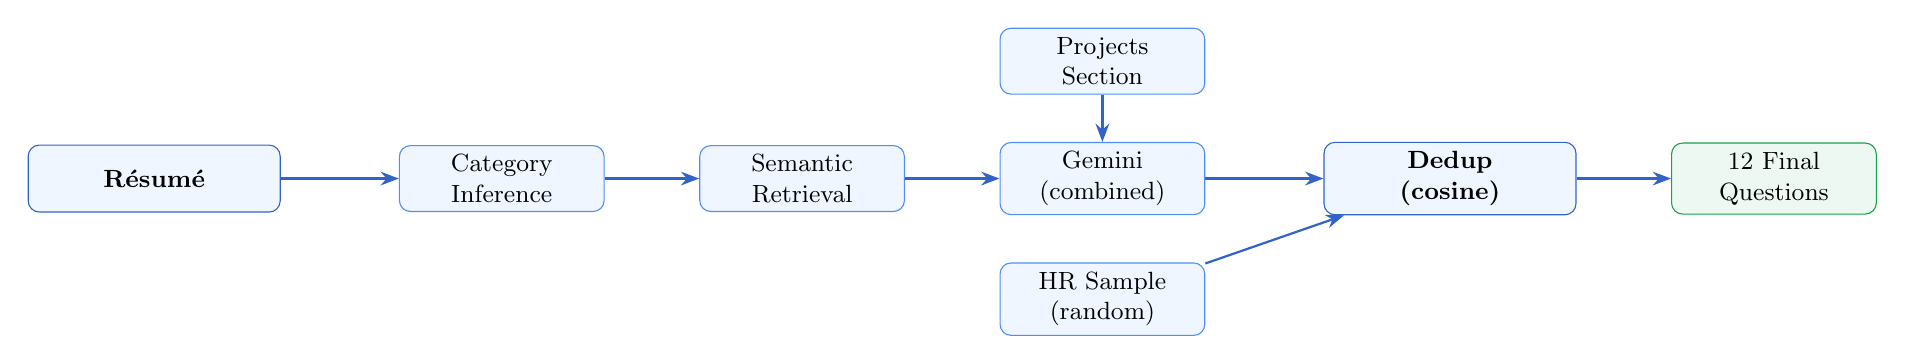
\begin{tikzpicture}[node distance=0.55cm and 0.3cm, every node/.style={font=\small}]
  \node[bigbox] (resume) {R\'esum\'e};
  \node[box, right=1.5cm of resume] (cats) {Category\\Inference};
  \node[box, right=1.2cm of cats] (retrieve) {Semantic\\Retrieval};
  \node[box, right=1.2cm of retrieve] (gemini) {Gemini\\(combined)};
  \node[box, above=0.6cm of gemini] (projects) {Projects\\Section};
  \node[box, below=0.6cm of gemini] (hr) {HR Sample\\(random)};
  \node[bigbox, right=1.5cm of gemini] (dedup) {Dedup\\(cosine)};
  \node[greenbox, right=1.2cm of dedup] (final) {12 Final\\Questions};

  \draw[arrow] (resume) -- (cats);
  \draw[arrow] (cats) -- (retrieve);
  \draw[arrow] (retrieve) -- (gemini);
  \draw[arrow] (projects) -- (gemini);
  \draw[arrow] (hr) -- (dedup);
  \draw[arrow] (gemini) -- (dedup);
  \draw[arrow] (dedup) -- (final);
\end{tikzpicture}
\caption{Question generation pipeline: three sources merged and deduplicated.}
\end{figure}

\subsection{Embedding Engine (\texttt{embedding\_engine.py})}

A TF-IDF vectorizer is fit on the full question bank at server startup:

\begin{itemize}[leftmargin=1.5em]
  \item \textbf{Vocabulary}: \texttt{max\_features=8000}, \texttt{ngram\_range=(1,2)}, English stop words removed.
  \item \textbf{Weighting}: \texttt{sublinear\_tf=True} (log TF), \texttt{min\_df=2}, \texttt{max\_df=0.95}.
  \item \textbf{Index}: FAISS \texttt{IndexFlatIP} over L2-normalized vectors (inner product = cosine for unit vectors).
  \item \textbf{Search}: \texttt{index.search(query\_vec, top\_k)} returns indices of nearest neighbors.
\end{itemize}

For smaller per-category corpora (typically 20--80 questions), a numpy dot-product rank is used instead of FAISS to avoid index rebuilding overhead.

\subsection{Answer Scoring (\texttt{gemini\_client.py}: \texttt{score\_answer})}

Each submitted answer is scored by Gemini with a structured prompt:

\begin{itemize}[leftmargin=1.5em]
  \item \textbf{Technical questions} (\texttt{has\_answer=true}): The model answer is included in the prompt. Gemini scores conceptual correctness, technical accuracy, and completeness relative to the expected answer.
  \item \textbf{Behavioral questions} (\texttt{has\_answer=false}): The prompt notes ``This is a behavioral question --- there is no model answer.'' Gemini scores effort/detail, use of specific examples, and STAR structure.
\end{itemize}

The prompt demands a JSON response with fields \texttt{overall} (0--100), \texttt{is\_behavioral}, \texttt{angles.conceptual/technical/completeness} (0--100 each), and \texttt{feedback} (1--2 sentences). All scores are clamped to [0, 100] server-side.

\textbf{Whisper-first scoring}: the \texttt{/api/confidence} call is made first and awaited blocking. The returned Whisper transcript replaces the lower-quality browser speech recognition text as input to Gemini, substantially improving scoring accuracy.

\subsection{Confidence Analysis Pipeline (\texttt{feature\_extractor.py})}

\begin{enumerate}[leftmargin=2em]
  \item \textbf{Receive audio}: webm blob from browser MediaRecorder.
  \item \textbf{Convert}: \texttt{AudioSegment.from\_file()} + \texttt{.export("temp.wav")} via pydub/ffmpeg.
  \item \textbf{Transcribe}: faster-whisper \texttt{medium.en} with \texttt{beam\_size=5}; device selection: CUDA float16 $\rightarrow$ CUDA int8 $\rightarrow$ CPU int8.
  \item \textbf{Extract 6 features} from WAV + transcript (see Table~\ref{tab:features}).
  \item \textbf{Predict}: load ensemble model from \texttt{.joblib}; \texttt{predict\_proba()[:, 1]} gives $P(\text{Confident})$.
  \item \textbf{Score}: $\text{score}_{1\text{--}10} = 1 + 9 \times P(\text{Confident})$.
  \item \textbf{Return}: \texttt{\{predicted\_label, confidence\_probability, confidence\_score\_1\_to\_10, transcript\}}.
  \item \textbf{Cleanup}: temporary directory deleted in \texttt{finally} block.
\end{enumerate}

\begin{table}[H]
\centering
\caption{Audio features extracted for confidence prediction}
\label{tab:features}
\small
\begin{tabularx}{\textwidth}{l l X}
\toprule
\textbf{Feature} & \textbf{Source} & \textbf{Computation} \\
\midrule
\texttt{filler\_words} & Transcript & Count of: um, uh, like, you know, so, basically, actually, literally \\
\texttt{speech\_rate} & Transcript + duration & $(\text{word\_count} / \text{duration\_s}) \times 60$ (words per minute) \\
\texttt{total\_repeated\_words} & Transcript & Count of consecutive identical words in token list \\
\texttt{total\_pauses} & WAV (pydub) & Number of silence segments $\geq 500$ ms; threshold = dBFS $-10$ \\
\texttt{average\_pause\_duration} & WAV (pydub) & Mean silence segment length in seconds \\
\texttt{pause\_per\_word} & Engineered & $\texttt{total\_pauses} / \texttt{speech\_rate}$ \\
\bottomrule
\end{tabularx}
\end{table}

\subsection{Text-to-Speech Integration}

SmartInterview supports two TTS providers selected by a single constant in \texttt{InterviewScreen.jsx}:

\begin{description}[leftmargin=2em]
  \item[\texttt{TTS\_PROVIDER = "elevenlabs"}] Calls \texttt{POST /api/tts} (FastAPI proxy to ElevenLabs API). Voice: Adam (\texttt{pNInz6obpgDQGcFmaJgB}), model: \texttt{eleven\_turbo\_v2}. Audio returned as MP3 blob, played via \texttt{new Audio()}.
  \item[\texttt{TTS\_PROVIDER = "browser"}] Web Speech Synthesis API with a voice priority chain: Microsoft Neural Natural $\rightarrow$ Microsoft Online $\rightarrow$ Microsoft Aria/Jenny/Guy $\rightarrow$ Google US $\rightarrow$ any en-US $\rightarrow$ any English. Rate: 0.88.
\end{description}

\subsection{Frontend State Management (\texttt{useInterview.js})}

All interview state lives in a single custom hook. Key design decisions:

\begin{itemize}[leftmargin=1.5em]
  \item \textbf{Answers dict} keyed by question ID allows random-order answering and O(1) lookup.
  \item \textbf{Confidence scores dict} separate from answers; populated asynchronously.
  \item \textbf{Blocking Whisper}: the confidence API call is \texttt{await}ed before the score API call. This ensures the Whisper transcript is available for scoring.
  \item \textbf{\texttt{hasAudio} gate}: submit is disabled until \texttt{MediaRecorder.onstop} fires and saves the blob, preventing submission of empty recordings.
  \item \textbf{Sequence counter (\texttt{seqRef})}: incremented on every question change or replay; async callbacks check \texttt{seqRef.current === seq} before executing, preventing stale state updates.
\end{itemize}

% ╔══════════════════════════════════════════════════════════╗
% ║  6. MACHINE LEARNING: CONFIDENCE ANALYSIS                ║
% ╚══════════════════════════════════════════════════════════╝
\section{Machine Learning: Confidence Analysis}

\subsection{Problem Statement}

Given a 5--60 second voice recording of an interview answer, classify the speaker as \textbf{Confident} (1) or \textbf{Unconfident} (0) and output a calibrated probability for a 1--10 score display.

\subsection{Dataset}
\label{sec:dataset}

Two data sources were combined:

\begin{description}[leftmargin=2em]
  \item[\texttt{audio\_features V3.csv}] --- An existing labeled dataset of audio features from voice recordings. Files are labeled \texttt{Confident} or \texttt{Unconfident}. Pre-filtering applied: average pitch 150--300 Hz, speech rate 60--220 WPM, and anomalous unconfident outliers (speech rate $>150$ WPM \textit{and} total pauses $<15$) removed.
  \item[\texttt{unconfident\_features.csv}] --- A custom dataset of 42 self-recorded unconfident voice messages (see Section~\ref{sec:augmentation}), with features extracted via the full feature extraction pipeline.
\end{description}

\textbf{Combined dataset}: 130 samples (shape: $130 \times 13$). Class distribution: 75 Confident, 55 Unconfident. Train/test split (80/20, stratified): train \{Confident: 60, Unconfident: 44\}, test \{Confident: 15, Unconfident: 11\}.

\subsection{Data Augmentation: Self-Recorded Samples}
\label{sec:augmentation}

The original dataset was heavily skewed toward confident samples. To correct this without synthetic oversampling, the developer self-recorded 42 voice messages designed to sound unconfident. The recording protocol:

\begin{enumerate}[leftmargin=2em]
  \item Scripted sentences covering common interview topics were prepared to ensure lexical diversity.
  \item Multiple takes per sentence were recorded (\texttt{sentence01\_take1}, \texttt{sentence01\_take2}, \ldots) creating a \texttt{sentence\_group} structure for cross-validation (see Section~\ref{sec:cv}).
  \item Recordings delivered in an intentionally hesitant, monotone, or filler-heavy manner.
  \item Audio saved as M4A voice messages, then batch-converted to WAV using pydub.
\end{enumerate}

\textbf{Feature extraction pipeline for self-recorded samples} (\texttt{UnconfidentVms\_Preprocess.ipynb}):

\begin{enumerate}[leftmargin=2em]
  \item Load WAV with librosa (22050 Hz, mono).
  \item Noise reduction: if RMS energy $< 0.01$, apply spectral subtraction via STFT.
  \item Transcribe with Whisper \texttt{base} model (English, FP16 on GPU).
  \item Extract pitch via \texttt{librosa.piptrack} (range 50--300 Hz).
  \item Compute pitch variability (std deviation of pitch frames).
  \item Detect pauses with WebRTC VAD (mode 3, 10 ms frames, 16 kHz mono).
  \item Count filler words using a 30-word list (broader than the production list) via Whisper \texttt{tiny} (more sensitive to fillers like ``um'', ``uh'').
  \item Compute speech rate from Whisper word count and librosa duration.
\end{enumerate}

\begin{warningbox}[Bias Discovery]
After merging the self-recorded samples, analysis revealed that the pitch features (\texttt{avg\_pitch}, \texttt{pitch\_variability}) were biased: the self-recorded voice had a distinct pitch signature that the model could exploit to trivially classify ``self-recorded = Unconfident'' rather than learning genuine confidence cues. This led to the \textbf{reduced feature set} (6 features, pitch removed) used for the final model.
\end{warningbox}

\subsection{Feature Sets}

\begin{table}[H]
\centering
\caption{Full vs.\ reduced feature sets}
\small
\begin{tabular}{l l c c}
\toprule
\textbf{Feature} & \textbf{Type} & \textbf{Full Set} & \textbf{Reduced Set} \\
\midrule
\texttt{filler\_words} & Linguistic & \checkmark & \checkmark \\
\texttt{avg\_pitch} & Acoustic & \checkmark & \texttimes \\
\texttt{pitch\_variability} & Acoustic & \checkmark & \texttimes \\
\texttt{speech\_rate} & Prosodic & \checkmark & \checkmark \\
\texttt{total\_repeated\_words} & Linguistic & \checkmark & \checkmark \\
\texttt{total\_pauses} & Temporal & \checkmark & \checkmark \\
\texttt{average\_pause\_duration} & Temporal & \checkmark & \checkmark \\
\texttt{pause\_per\_word} & Engineered & \checkmark & \checkmark \\
\bottomrule
\end{tabular}
\end{table}

\subsection{Cross-Validation Strategy}
\label{sec:cv}

Standard stratified k-fold was avoided because the dataset contains multiple takes of the same sentence by the same speaker. Using \texttt{GroupKFold} ensures that all takes of a sentence are in the same fold, preventing data leakage:

\begin{lstlisting}[style=python, numbers=none]
gkf = GroupKFold(n_splits=5)
scores = cross_val_score(pipeline, X, y, cv=gkf,
                         groups=sentence_group, scoring='roc_auc')
\end{lstlisting}

Unique groups: 91 train, 23 test (total 114 sentence groups).

\subsection{Models Evaluated}
\label{sec:models}

All models were built as scikit-learn \texttt{Pipeline} objects:
\texttt{SimpleImputer(strategy='mean')} $\rightarrow$ \texttt{StandardScaler} $\rightarrow$ \textit{classifier}.

\subsubsection{Full Feature Set Results}

\begin{table}[H]
\centering
\caption{GroupKFold cross-validation ROC-AUC (full 8-feature set)}
\small
\begin{tabular}{l c c c c}
\toprule
\textbf{Model} & \textbf{CV AUC} & \textbf{$\pm$ Std} & \textbf{Test Acc.} & \textbf{Test AUC} \\
\midrule
Logistic Regression & 0.890 & 0.044 & 88\% & 0.939 \\
Random Forest (n=100) & 0.858 & 0.062 & --- & --- \\
XGBoost & 0.849 & 0.036 & --- & --- \\
AdaBoost (n=50) & 0.847 & 0.093 & --- & --- \\
\midrule
\multicolumn{5}{l}{\textit{Best single model: Logistic Regression}} \\
\bottomrule
\end{tabular}
\end{table}

Full-set Logistic Regression test classification report:
\begin{lstlisting}[numbers=none]
              precision  recall  f1-score  support
Unconfident       0.83    0.91      0.87       11
  Confident       0.93    0.87      0.90       15
   accuracy                         0.88       26
\end{lstlisting}

\subsubsection{Reduced Feature Set Results (Pitch Removed)}

\begin{table}[H]
\centering
\caption{GroupKFold cross-validation ROC-AUC (reduced 6-feature set)}
\small
\begin{tabular}{l c c c c}
\toprule
\textbf{Model} & \textbf{CV AUC} & \textbf{$\pm$ Std} & \textbf{Test Acc.} & \textbf{Test AUC} \\
\midrule
Logistic Regression & 0.843 & 0.044 & 85\% & 0.952 \\
Random Forest (n=100) & 0.842 & 0.035 & 92\% & 0.903 \\
XGBoost (tuned) & 0.832 & 0.032 & 92\% & 0.903 \\
AdaBoost (n=50) & 0.799 & 0.074 & 92\% & 0.955 \\
\bottomrule
\end{tabular}
\end{table}

Reduced-feature Random Forest / AdaBoost test report (identical results):
\begin{lstlisting}[numbers=none]
              precision  recall  f1-score  support
Unconfident       1.00    0.82      0.90       11
  Confident       0.88    1.00      0.94       15
   accuracy                         0.92       26
\end{lstlisting}

\subsection{Hyperparameter Tuning (XGBoost)}

\texttt{GridSearchCV} with GroupKFold (5 folds) was run over 108 combinations:

\begin{lstlisting}[style=python, numbers=none]
param_grid = {
    'model__n_estimators':    [50, 100, 200],
    'model__max_depth':       [3, 5, 7],
    'model__learning_rate':   [0.01, 0.1, 0.2],
    'model__subsample':       [0.7, 0.9],
    'model__colsample_bytree':[0.7, 0.9],
}
\end{lstlisting}

\textbf{Best parameters}: \texttt{colsample\_bytree=0.7, learning\_rate=0.01, max\_depth=5, n\_estimators=50, subsample=0.7}. Best CV AUC: 0.891.

\subsection{Ensemble Model: Final Architecture}

The final deployed model is a \texttt{VotingClassifier} (soft voting, equal weights) over the four \textit{reduced-feature} pipelines:

\begin{lstlisting}[style=python, numbers=none]
ensemble = VotingClassifier(
    estimators=[
        ('lr',  lr_pipeline_reduced),
        ('rf',  rf_pipeline_reduced),
        ('xgb', xgb_pipeline_reduced),
        ('ada', ada_pipeline_reduced),
    ],
    voting='soft',   # average predicted probabilities
    weights=[1, 1, 1, 1],
    n_jobs=-1,
)
\end{lstlisting}

\textbf{Rationale for ensemble}: No single model dominated across all metrics. Soft voting averages the probability estimates from four models with diverse inductive biases (linear, tree-bagging, gradient boosting, adaptive boosting), reducing variance without sacrificing the accuracy of the stronger individual models.

\textbf{Ensemble test results}:
\begin{lstlisting}[numbers=none]
              precision  recall  f1-score  support
Unconfident       0.90    0.82      0.86       11
  Confident       0.88    0.93      0.90       15
   accuracy                         0.88       26
   ROC-AUC:  0.927
\end{lstlisting}

\subsection{Overfitting Analysis}

\begin{table}[H]
\centering
\caption{CV AUC vs.\ test AUC comparison (no overfitting detected)}
\small
\begin{tabular}{l c c}
\toprule
\textbf{Model} & \textbf{CV AUC} & \textbf{Test AUC} \\
\midrule
Full Feature Logistic Regression & 0.890 & 0.939 \\
Reduced Feature Logistic Regression & 0.843 & 0.952 \\
\bottomrule
\end{tabular}
\end{table}

Test AUCs exceed CV AUCs slightly, consistent with normal statistical variation on a 26-sample test set. No overfitting is indicated.

\subsection{Model Serialization}

After training, the ensemble and feature name list are saved with \texttt{joblib}:

\begin{lstlisting}[style=python, numbers=none]
joblib.dump(ensemble_model, 'ensemble_confidence_model.joblib')
joblib.dump(FEATURES_REDUCED, 'features_list.joblib')
\end{lstlisting}

At runtime, \texttt{feature\_extractor.py} loads these files lazily on first request. The Whisper model is also loaded lazily and cached in a module-level global.

% ╔══════════════════════════════════════════════════════════╗
% ║  7. CHALLENGES & SOLUTIONS                               ║
% ╚══════════════════════════════════════════════════════════╝
\section{Challenges and Solutions}

\subsection{Small Dataset and Class Imbalance}

\textbf{Challenge}: The initial dataset contained significantly more Confident samples than Unconfident. Standard oversampling (SMOTE) was considered but rejected because the features are real-valued audio measurements for which synthetic interpolation may not produce realistic patterns.

\textbf{Solution}: The developer self-recorded 42 unconfident voice messages speaking scripted sentences in a hesitant manner. This approach generates real acoustic patterns rather than interpolated feature vectors. The \texttt{sentence\_group} structure added for GroupKFold CV prevents these correlated samples from leaking across train/test splits.

\textbf{Residual limitation}: All unconfident samples in the augmented set come from a single speaker (the developer). The model may not generalize well to speakers with naturally hesitant speech patterns that differ from this recording style.

\subsection{Pitch Bias from Self-Recorded Samples}

\textbf{Challenge}: After augmentation, the pitch features (\texttt{avg\_pitch}, \texttt{pitch\_variability}) were found to be biased --- the self-recorded samples had a distinct pitch signature that correlated with the unconfident label independent of actual confidence. This was discovered by comparing model performance on the full vs.\ reduced feature sets and noting that the drop in CV AUC was larger than expected if pitch were a genuinely informative feature.

\textbf{Solution}: Both pitch features were dropped entirely. The reduced 6-feature set performs slightly worse on CV AUC (0.843 vs.\ 0.890) but is more robust to speaker-dependent pitch differences. The developer explicitly acknowledged this trade-off in the notebook.

\subsection{Browser Speech Recognition Inaccuracy}

\textbf{Challenge}: The original implementation sent browser Web Speech API transcripts to Gemini for scoring. Browser SR is known to perform poorly on technical vocabulary (``FAISS'', ``cosine similarity'', ``hyperparameter'', API names). Scored answers were consistently rated low because the transcript misrepresented what the candidate said.

\textbf{Solution}: The confidence analysis endpoint (\texttt{/api/confidence}) already transcribed audio with faster-whisper \texttt{medium.en}. The endpoint was modified to return the transcript alongside confidence scores. The \texttt{submitAnswer} hook now awaits the confidence call first (blocking) and uses the Whisper transcript as input to Gemini scoring. Browser SR continues to run silently as a fallback ref.

\subsection{Gemini Quota and Model Availability}

\textbf{Challenge}: Question generation and answer scoring both call Gemini; heavy use quickly exhausts the free tier quota. Additionally, the \texttt{gemini-1.5-flash} model ID was deprecated in the v1beta API and returns a 404 error.

\textbf{Solution}: The model name is configured via the \texttt{GEMINI\_MODEL} environment variable; the default was changed to \texttt{gemini-2.0-flash}, which has a higher free-tier quota and is available in v1beta. The \texttt{load\_dotenv(override=True)} call ensures \texttt{.env} changes take effect even when a prior environment variable was already loaded in the process.

\subsection{Async Audio Submission Race Condition}

\textbf{Challenge}: \texttt{MediaRecorder.onstop} is asynchronous; calling \texttt{mediaRecorder.stop()} does not synchronously make the audio blob available. Early implementations tried to access the blob immediately after \texttt{stop()}, resulting in empty submissions.

\textbf{Solution}: A \texttt{wantBlobRef} boolean ref is used as a handshake. \texttt{stopSequence()} resets \texttt{wantBlobRef.current = false} synchronously, then immediately sets it to \texttt{true}. When \texttt{onstop} fires asynchronously, it sees \texttt{wantBlobRef.current === true} and saves the blob, then sets \texttt{hasAudio(true)} to enable the submit button.

\subsection{ElevenLabs Voice Tier Restrictions}

\textbf{Challenge}: Several voice IDs attempted during development (Rachel, Josh) returned HTTP 402 errors because they belong to the ``Voice Library'' tier, which requires a paid plan.

\textbf{Solution}: Switched to the Adam voice (\texttt{pNInz6obpgDQGcFmaJgB}), which is a ``Premade'' voice available on the free tier. Voice ID is configurable via \texttt{ELEVENLABS\_VOICE\_ID} in \texttt{.env}. Browser TTS remains the default provider to avoid any cost dependency for development.

% ╔══════════════════════════════════════════════════════════╗
% ║  8. KEY INSIGHTS & ERROR ANALYSIS                        ║
% ╚══════════════════════════════════════════════════════════╝
\section{Key Insights and Error Analysis}

\subsection{ML Model Insights}

\begin{infobox}[Logistic Regression dominates on full features]
Despite being the simplest model, LR achieved the highest CV AUC (0.890) on the full feature set. This suggests the confidence signal in these 8 features is largely linearly separable. Tree-based models did not benefit from the additional non-linearity on this small dataset.
\end{infobox}

\begin{infobox}[Reduced features hurt LR more than trees]
On the reduced set, LR dropped by 4.7 points (0.890 $\rightarrow$ 0.843), while RF and XGBoost dropped by only 1.6 and 1.7 points respectively. The pitch features were apparently more informative for the linear boundary. Trees captured non-linear combinations of the remaining features more effectively.
\end{infobox}

\begin{infobox}[Soft voting preserves calibration]
The ensemble uses soft voting (average probabilities) rather than hard voting (majority label). This produces calibrated probability estimates suitable for the 1--10 score mapping ($1 + 9P$). Hard voting would collapse probabilities to 0/1 and lose granularity.
\end{infobox}

\subsection{Sample-Level Error Analysis}

On the 26-sample test set, the ensemble misclassified 3 samples:
\begin{itemize}[leftmargin=1.5em]
  \item \textbf{2 Unconfident predicted as Confident}: These had relatively high speech rates and low pause counts, which the reduced-feature model associates with confidence. Likely cases where the speaker spoke quickly due to nervousness rather than fluency.
  \item \textbf{1 Confident predicted as Unconfident}: High filler-word count despite an otherwise confident delivery. The filler-word feature is a blunt instrument that penalizes casual speech.
\end{itemize}

\subsection{System-Level Insights}

\begin{itemize}[leftmargin=1.5em]
  \item \textbf{RAG is necessary but not sufficient}: Pure LLM question generation produces coherent but generic questions. The dataset retrieval step grounds questions in domain knowledge and difficulty distribution; Gemini then personalizes them to the candidate. Neither alone achieves the desired specificity.
  \item \textbf{Whisper \texttt{medium.en} is the right model for interview audio}: The \texttt{small} model (previously used) struggled with technical terminology. The \texttt{medium.en} model correctly transcribed domain terms in testing, justifying the higher computational cost.
  \item \textbf{Per-question score display is counterproductive}: Showing scores immediately after each answer disrupted the interview flow and caused anxiety. Scores are now shown only in the final report, matching the real interview experience.
  \item \textbf{Gemini model selection matters significantly}: \texttt{gemini-2.5-flash} produces higher-quality question personalization and more nuanced scoring feedback than \texttt{gemini-2.0-flash}, but exhausts the free-tier quota approximately 3$\times$ faster.
\end{itemize}

% ╔══════════════════════════════════════════════════════════╗
% ║  9. SETUP & REPRODUCTION INSTRUCTIONS                    ║
% ╚══════════════════════════════════════════════════════════╝
\section{Setup and Reproduction Instructions}

\subsection{Prerequisites}

\begin{itemize}[leftmargin=1.5em]
  \item Python 3.12+ and pip
  \item Node.js 18+ and npm
  \item ffmpeg installed and on PATH (required by pydub)
  \item A Google Gemini API key (\href{https://aistudio.google.com}{aistudio.google.com})
  \item (Optional) An ElevenLabs API key for realistic TTS
\end{itemize}

\subsection{Backend Setup}

\begin{lstlisting}[style=bash, numbers=none]
# 1. Clone / navigate to the project root
cd SmartInterview/backend

# 2. Create and activate virtual environment
python -m venv venv
# Windows:
venv\Scripts\activate
# macOS / Linux:
source venv/bin/activate

# 3. Install dependencies
pip install -r requirements.txt

# 4. Download spaCy model
python -m spacy download en_core_web_sm

# 5. Configure environment
# Create backend/.env with:
#   GEMINI_API_KEY=AIzaSy...
#   GEMINI_MODEL=gemini-2.0-flash
#   ELEVENLABS_API_KEY=sk_...     (optional)
#   ELEVENLABS_VOICE_ID=pNInz6obpgDQGcFmaJgB  (optional, Adam)

# 6. Verify model files exist
# backend/models/ensemble_confidence_model.joblib
# backend/models/features_list.joblib
# backend/data/master_questions.csv

# 7. Start the server
uvicorn main:app --reload --port 8000
\end{lstlisting}

\subsection{Frontend Setup}

\begin{lstlisting}[style=bash, numbers=none]
cd SmartInterview/frontend

# Install dependencies
npm install

# Start dev server (proxies /api -> http://localhost:8000)
npm run dev
# Browser: http://localhost:5173
\end{lstlisting}

\subsection{Reproducing the Confidence Model}

To retrain the ensemble model from scratch:

\begin{enumerate}[leftmargin=2em]
  \item Prepare \texttt{audio\_features V3.csv} (original dataset with Confident/Unconfident labels and feature columns matching the schema in Section~\ref{sec:dataset}).
  \item Run \texttt{UnconfidentVms\_Preprocess.ipynb} in Google Colab to process self-recorded unconfident voice messages and produce \texttt{unconfident\_features.csv}.
  \item Run \texttt{ConfidenceAnalysis.ipynb} in Google Colab. The notebook will:
  \begin{enumerate}
    \item Filter and merge both datasets (130 samples total).
    \item Engineer the \texttt{pause\_per\_word} feature.
    \item Build sentence groupings for GroupKFold CV.
    \item Train and evaluate LR, RF, XGBoost, AdaBoost on both feature sets.
    \item Run XGBoost GridSearchCV (108 hyperparameter combinations).
    \item Train the VotingClassifier ensemble on the reduced feature set.
    \item Save \texttt{ensemble\_confidence\_model.joblib} and \texttt{features\_list.joblib}.
  \end{enumerate}
  \item Download the two \texttt{.joblib} files from Google Drive to \texttt{backend/models/}.
\end{enumerate}

\subsection{Environment Variables Reference}

\begin{table}[H]
\centering
\caption{Backend environment variables}
\small
\begin{tabularx}{\textwidth}{l l X}
\toprule
\textbf{Variable} & \textbf{Required} & \textbf{Description} \\
\midrule
\texttt{GEMINI\_API\_KEY} & Yes & Google Gemini API key from AI Studio \\
\texttt{GEMINI\_MODEL} & No & Default: \texttt{gemini-2.0-flash} \\
\texttt{ELEVENLABS\_API\_KEY} & No & ElevenLabs key (TTS only) \\
\texttt{ELEVENLABS\_VOICE\_ID} & No & Default: \texttt{pNInz6obpgDQGcFmaJgB} (Adam) \\
\texttt{CONFIDENCE\_MODEL\_PATH} & No & Default: \texttt{backend/models/ensemble\_confidence\_model.joblib} \\
\texttt{CONFIDENCE\_FEATURES\_PATH} & No & Default: \texttt{backend/models/features\_list.joblib} \\
\texttt{DATA\_PATH} & No & Default: \texttt{data/master\_questions.csv} \\
\texttt{CORS\_ORIGINS} & No & Default: \texttt{http://localhost:5173} \\
\bottomrule
\end{tabularx}
\end{table}

% ╔══════════════════════════════════════════════════════════╗
% ║  10. CONCLUSION & LIMITATIONS                            ║
% ╚══════════════════════════════════════════════════════════╝
\section{Conclusion and Limitations}

\subsection{Summary of Contributions}

SmartInterview demonstrates that a practical, personalized interview preparation tool can be built by composing off-the-shelf AI components (Gemini, Whisper, FAISS) with a custom ensemble ML model trained on self-collected data. The system addresses the cold-start problem of question generation (no prior interview data needed) by using the candidate's r\'esum\'e as a RAG retrieval signal, and the scoring problem by delegating evaluation to an LLM with structured output constraints.

The original research contribution is the self-recorded unconfident voice dataset and the resulting analysis of how speaker-specific acoustic bias (pitch) can corrupt a small-data classifier. The decision to drop pitch features in favor of a less accurate but more generalizable model reflects practical data science judgment.

\subsection{Known Limitations}

\begin{enumerate}[leftmargin=2em]
  \item \textbf{Confidence model dataset size}: 130 samples from a limited number of speakers is insufficient for a robust production model. The model is likely to generalize poorly to speakers with significantly different accents or speaking styles.
  \item \textbf{Single-speaker augmentation}: All 42 self-recorded unconfident samples come from one speaker. The model has never seen unconfident speech from any other speaker.
  \item \textbf{Feature shallowness}: The 6 features are hand-crafted. Deep audio features (MFCCs, spectral centroid, mel-spectrogram embeddings via a pre-trained model) could capture richer confidence signals.
  \item \textbf{No session persistence}: The in-memory session store is lost on server restart. A Redis or database backend would be needed for production.
  \item \textbf{Gemini quota dependency}: Both question generation and answer scoring call the Gemini API. Rate limits make the system unreliable under heavy concurrent use without caching.
  \item \textbf{Resume parser brittleness}: The regex-based section detector fails on non-standard layouts (two-column, tables, graphics-heavy PDFs). A dedicated document AI service would improve reliability.
  \item \textbf{ElevenLabs cost}: Realistic TTS requires a paid ElevenLabs plan for voices outside the free-tier premade set. The browser TTS fallback is functional but less natural-sounding.
\end{enumerate}

\subsection{Potential Future Work}

\begin{itemize}[leftmargin=1.5em]
  \item Replace TF-IDF embeddings with a sentence-transformer model (e.g., \texttt{all-MiniLM-L6-v2}) for more semantic retrieval.
  \item Collect a larger, more diverse confidence dataset or use a pre-trained speech emotion recognition model as a base.
  \item Add a PostgreSQL/Redis backend for session persistence and concurrent user support.
  \item Implement caching for Gemini responses keyed on (resume hash, role, JD hash) to reduce quota consumption across similar sessions.
  \item Explore fine-tuning Whisper \texttt{small} on interview-domain vocabulary to reduce compute cost while maintaining accuracy.
\end{itemize}

% ╔══════════════════════════════════════════════════════════╗
% ║  APPENDIX                                                ║
% ╚══════════════════════════════════════════════════════════╝
\appendix

\section{Question Bank Schema}

\begin{table}[H]
\centering
\caption{\texttt{master\_questions.csv} column schema}
\small
\begin{tabular}{l l l}
\toprule
\textbf{Column} & \textbf{Type} & \textbf{Description} \\
\midrule
\texttt{id} & string & Unique question identifier \\
\texttt{category} & string & One of 11 canonical categories \\
\texttt{question} & string & Question text \\
\texttt{answer} & string/null & Model answer; NULL for behavioral questions \\
\texttt{difficulty} & string & Easy / Medium / Hard \\
\texttt{source} & string & Dataset source name \\
\texttt{has\_answer} & boolean & False when \texttt{answer} is NULL \\
\bottomrule
\end{tabular}
\end{table}

\section{Canonical Interview Categories}

\begin{enumerate}[leftmargin=2em]
  \item AI \& Data Science
  \item Software Engineering
  \item SQL \& Databases
  \item Cloud \& Containers
  \item DevOps
  \item DSA \& Algorithms
  \item Operating Systems
  \item Computer Networks
  \item Distributed Systems
  \item Concurrency
  \item HR \& Behavioral
\end{enumerate}

\section{Gemini Prompt Templates}

\subsection{Combined Question Generation Prompt (excerpt)}

\begin{lstlisting}[numbers=none, basicstyle=\ttfamily\footnotesize]
Complete TWO tasks in a single response:

TASK 1 - Personalize {dataset_count} template questions:
- Keep core concept, category, difficulty
- Reference candidate's actual project/technology/decision
- Update model answer with candidate context (2-3 sentences)

TASK 2 - Generate {project_count} new project questions:
- Target specific technical decision from a named project
- Must not overlap with Task 1 topics
- Model answer: 2-3 sentences from project detail

Return ONLY valid JSON: {"dataset": [...], "project": [...]}
\end{lstlisting}

\subsection{Answer Scoring Prompt (excerpt)}

\begin{lstlisting}[numbers=none, basicstyle=\ttfamily\footnotesize]
Question: {question}
Category: {category}
{answer_context}      <- model answer OR "behavioral, no model answer"
Candidate's Answer: {user_answer}

Return ONLY valid JSON:
{
  "overall": <0-100>,
  "is_behavioral": <bool>,
  "angles": {"conceptual": <0-100>, "technical": <0-100>,
              "completeness": <0-100>},
  "feedback": "<1-2 sentences>"
}
\end{lstlisting}

\section{Frontend Component Responsibilities}

\begin{table}[H]
\centering
\caption{Frontend component overview}
\small
\begin{tabularx}{\textwidth}{l X}
\toprule
\textbf{Component} & \textbf{Responsibility} \\
\midrule
\texttt{App.jsx} & Root routing; step indicator; loading screens with motivational quotes \\
\texttt{useInterview.js} & All interview state; API call orchestration; derived values \\
\texttt{api.js} & Axios instance; typed API call functions; error extraction \\
\texttt{UploadScreen.jsx} & Drag-and-drop file upload with mime/size validation \\
\texttt{ReadyScreen.jsx} & Optional role/JD input; scoring method explainer \\
\texttt{InterviewScreen.jsx} & TTS dispatch; countdown; MediaRecorder; submit gating \\
\texttt{ReportScreen.jsx} & Final report: overall score, category bars, per-question detail \\
\texttt{ProfileStrip.jsx} & Sticky strip: name, skills, weighted category pills \\
\texttt{ConfidenceTestPage.jsx} & Standalone confidence analyzer for calibration/testing \\
\texttt{QuestionsPage.jsx} & Read-only question preview with expandable model answers \\
\bottomrule
\end{tabularx}
\end{table}

\end{document}
